\documentclass[conference]{IEEEtran}
\IEEEoverridecommandlockouts
% The preceding line is only needed to identify funding in the first footnote. If that is unneeded, please comment it out.
\usepackage{cite}
\usepackage{amsmath,amssymb,amsfonts}
\usepackage{algorithm}
\usepackage{arevmath}     % For math symbols
\usepackage[noend]{algpseudocode}
\usepackage{graphicx}
\usepackage{textcomp}
\usepackage{xcolor}
\def\BibTeX{{\rm B\kern-.05em{\sc i\kern-.025em b}\kern-.08em
    T\kern-.1667em\lower.7ex\hbox{E}\kern-.125emX}}
\begin{document}

\title{Using AI in Integrated Navigation*\\
{\footnotesize \textsuperscript{*}Integrated Navigation Course Project Report}
}

\author{\IEEEauthorblockN{Ali Baniasad}
\IEEEauthorblockA{\textit{Department of Aerospace Engineering} \\
\textit{Sharif University of Technology}\\
Tehran, Iran \\
ali\_baniasad@ae.sharif.edu}
\and
\IEEEauthorblockN{Alireza Sharifi}
\IEEEauthorblockA{\textit{Department of Aerospace Engineering} \\
\textit{Sharif University of Technology}\\
Tehran, Iran \\
ar.sharifi@sharif.edu}
}

\maketitle

\begin{abstract}
    In this paper, we present an AI method which improve integrated navigation system performance. We use a deep neural network to estimate the error of the inertial navigation system. The network is trained by a LSTM network. The results show that the proposed method can improve the performance of the integrated navigation system. Three methods are proposed to train the network. The first method is to train the network by measurement update. The second method is to train the network by propagation and measurement to predict the attitude. The third one is used to predict attitude and heading in the absent of magnetometer or GPS. The results show that the proposed method can improve the performance of the navigation in absent of magnetometer or GPS. 
\end{abstract}

\begin{IEEEkeywords}
    Integrated Navigation, Deep Learning, LSTM, AI, Kalman Filter, AHRS
\end{IEEEkeywords}

\section{Introduction}
    Integrated navigation is a method to improve the performance of navigation system by using different sensors. In this method, the navigation system uses the information of different sensors to estimate the state of the system. The most common sensors used in integrated navigation are inertial measurement unit (IMU), magnetometer, GPS, and barometer. The IMU is used to estimate the attitude and position of the system. The magnetometer is used to estimate the heading of the system. The GPS is used to estimate the position of the system. The barometer is used to estimate the altitude of the system. The integrated navigation system uses the information of different sensors to estimate the state of the system. The most common method to estimate the state of the system is Kalman filter. The Kalman filter is a recursive filter which uses the information of different sensors to estimate the state of the system.



    \section{Attitude Heading Reference System (AHRS)}

    The Attitude Heading Reference System (AHRS) employing an Extended Kalman Filter (EKF) is a sophisticated method for accurate orientation estimation. This system integrates sensor measurements, such as accelerometers, gyroscopes, and optionally, magnetometer or GPS data, to provide robust attitude and heading information.
    \begin{algorithm}
        \caption{AHRS EKF Formulas with Euler Angles}
        \begin{algorithmic}[1]
          \Procedure{PredictionStep}{}
            \State \textbf{Input:} $\boldsymbol{\theta}$, $\boldsymbol{\omega}$, $\Delta t$, $\mathbf{P}$, $\mathbf{Q}$
            \State $\boldsymbol{\theta} \gets \text{EulerUpdate}(\boldsymbol{\theta}, \boldsymbol{\omega}, \Delta t)$
            \State $\mathbf{F} \gets \text{ComputeStateTransitionMatrix}(\boldsymbol{\theta}, \boldsymbol{\omega}, \Delta t)$
            \State $\mathbf{P} \gets \mathbf{F} \cdot \mathbf{P} \cdot \mathbf{F}^T + \mathbf{Q}$
          \EndProcedure
      
          \Procedure{CorrectionStep}{}
            \State \textbf{Input:} $\boldsymbol{\theta}$, $\mathbf{P}$, $\mathbf{H}$, $\mathbf{R}$, $\mathbf{K}$, $\mathbf{z}$, $\mathbf{h}$
            \State $\mathbf{K} \gets \mathbf{P} \cdot \mathbf{H}^T \cdot (\mathbf{H} \cdot \mathbf{P} \cdot \mathbf{H}^T + \mathbf{R})^{-1}$
            \State $\boldsymbol{\theta} \gets \text{EulerCorrection}(\boldsymbol{\theta}, \mathbf{K}, \mathbf{z} - \mathbf{h})$
            \State $\mathbf{P} \gets (\mathbf{I} - \mathbf{K} \cdot \mathbf{H}) \cdot \mathbf{P}$
          \EndProcedure
        \end{algorithmic}
    \end{algorithm}
          



\section{Network Filtering Measurements}
    In this section, we present a method to improve the performance of the integrated navigation system. In this method, we use a deep neural network to filter the measurements of the sensors. In this scenario gyroscope had time-variant bias. Here is the results and comparison of the performance of the integrated navigation system with and without the proposed method. The results show that the proposed method can improve the performance of the integrated navigation system. Here is the structure of the network. The network is trained by a LSTM network.
    \begin{figure}[H]
        \centerline{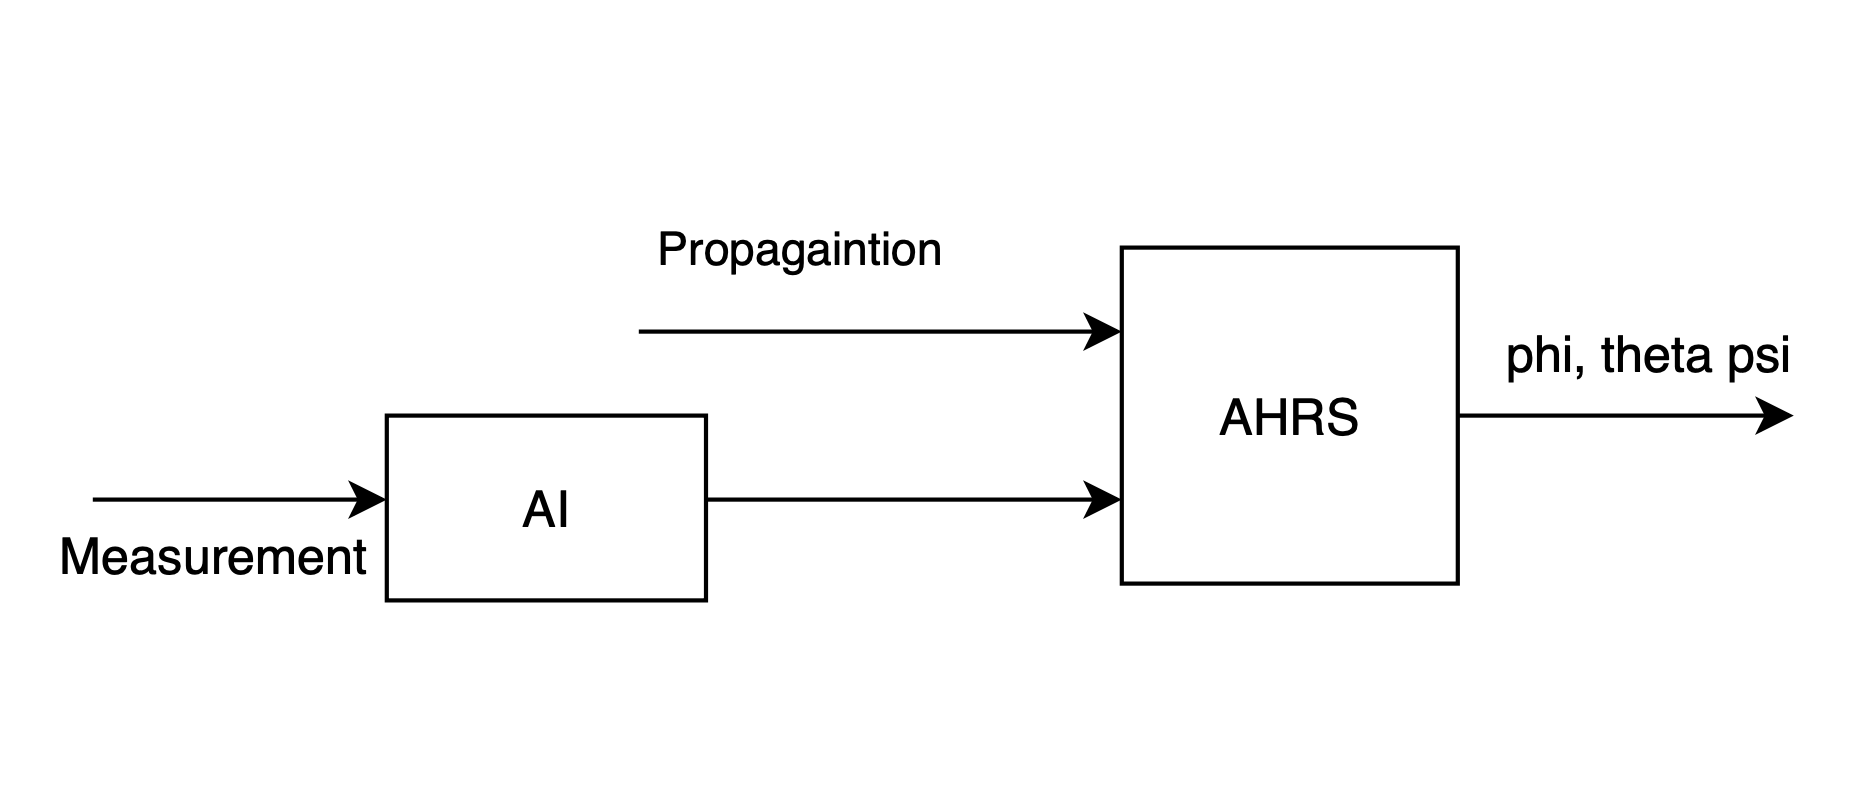
\includegraphics[width=0.5\textwidth]{../Figures/part_1_network.png}}
        \caption{Structure of the network method I.}
    \end{figure}
    \begin{figure}[H]
        \centerline{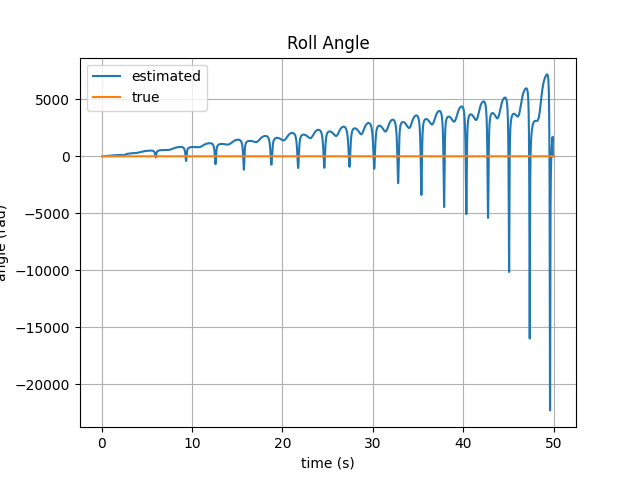
\includegraphics[width=0.5\textwidth]{../Figures/part_1_roll_no_AI.png}}
        \caption{Roll angle without AI.}
    \end{figure}
    \begin{figure}[H]
        \centerline{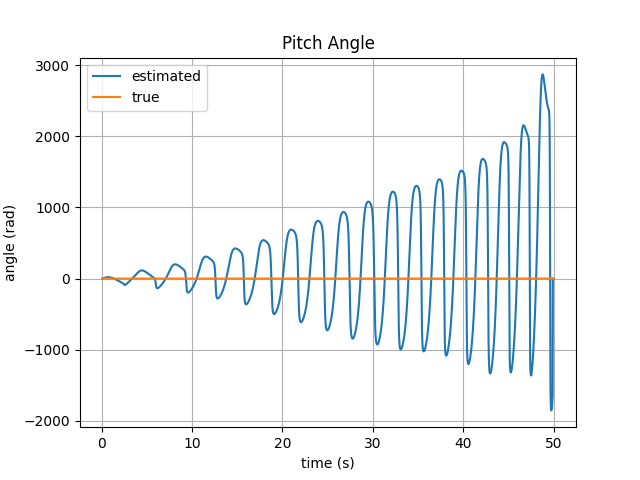
\includegraphics[width=0.5\textwidth]{../Figures/part_1_pitch_no_AI.png}}
        \caption{Pitch angle without AI.}
    \end{figure}
    \begin{figure}[H]
        \centerline{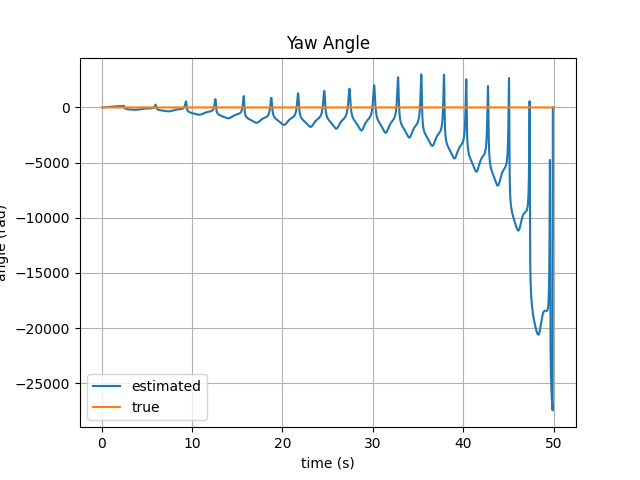
\includegraphics[width=0.5\textwidth]{../Figures/part_1_yaw_no_AI.png}}
        \caption{Yaw angle without AI.}
    \end{figure}
    \begin{figure}[H]
        \centerline{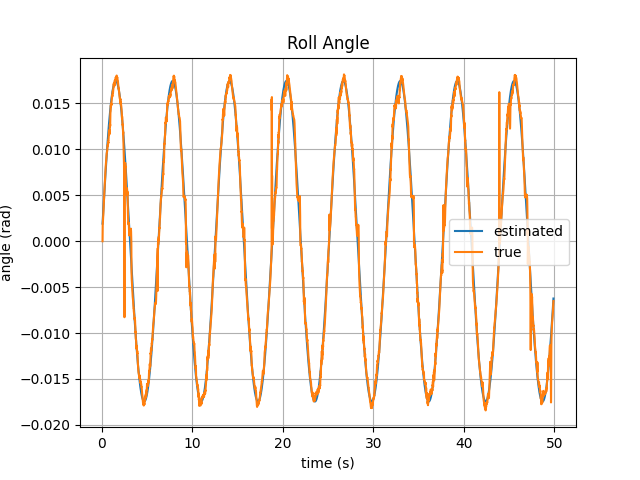
\includegraphics[width=0.5\textwidth]{../Figures/part_1_roll_AI.png}}
        \caption{Roll angle with AI.}
    \end{figure}
    \begin{figure}[H]
        \centerline{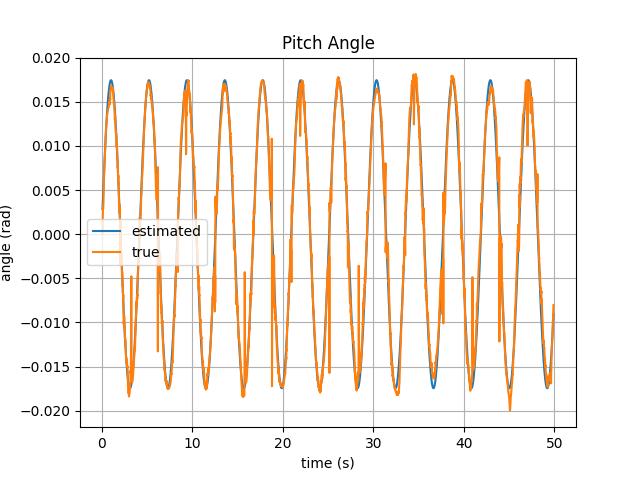
\includegraphics[width=0.5\textwidth]{../Figures/part_1_pitch_AI.png}}
        \caption{Pitch angle with AI.}
    \end{figure}
    \begin{figure}[H]
        \centerline{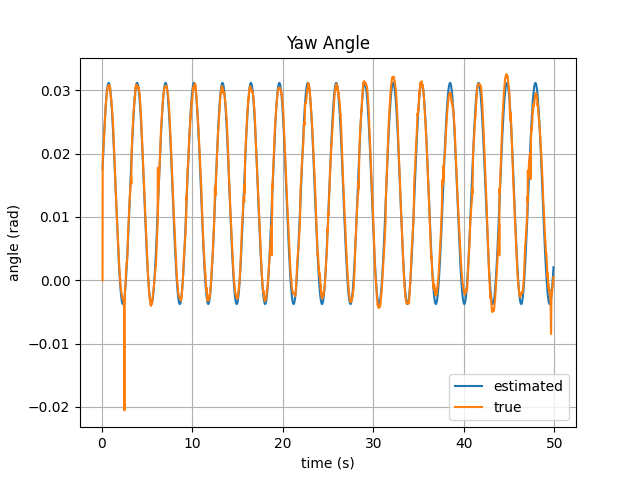
\includegraphics[width=0.5\textwidth]{../Figures/part_1_yaw_AI.png}}
        \caption{Yaw angle with AI.}
    \end{figure}
    
    \section{Network calculating attitude}
    In this section, we present a method to improve the performance of the integrated navigation system. In this method, we use a deep neural network to calculate the attitude of the system. In this scenario gyroscope had time-variant bias. Here is the results and comparison of the performance of the integrated navigation system with and without the proposed method. The results show that the proposed method can improve the performance of the integrated navigation system. Here is the structure of the network. The network is trained by a LSTM network.
    \begin{figure}[H]
        \centerline{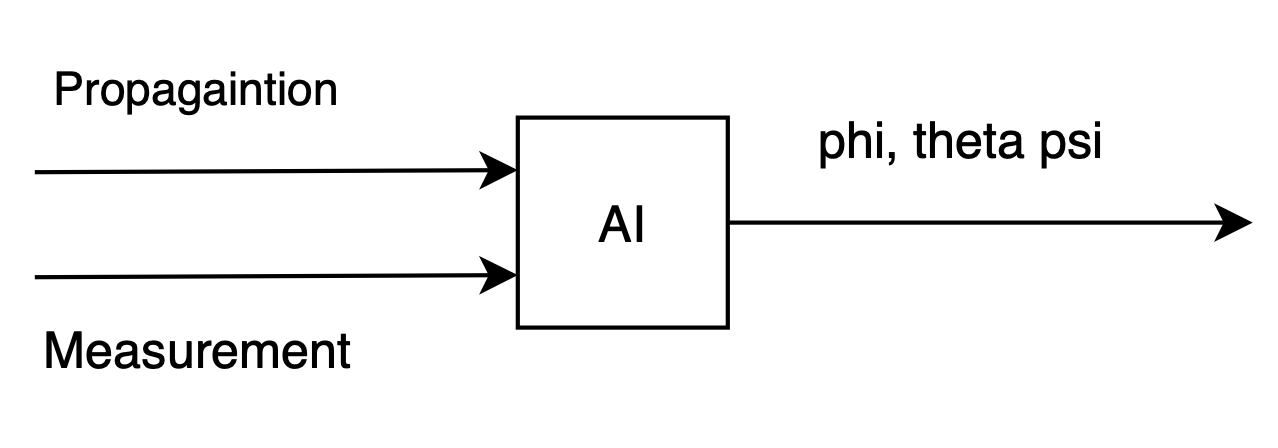
\includegraphics[width=0.5\textwidth]{../Figures/part_2_network.png}}
        \caption{Structure of the network method II.}
    \end{figure}
    

\end{document}
